\documentclass[10pt]{article}
\usepackage[margin=1in]{geometry}
\usepackage{amsmath,amssymb,graphicx,booktabs}
% Standard-font fallbacks for the local TeX installation.
\DeclareFontShape{OT1}{cmr}{m}{n}{<->cmr10}{}
\DeclareFontShape{OT1}{cmr}{bx}{n}{<->cmbx10}{}
\DeclareMathSizes{8}{10}{7}{7}
\DeclareMathSizes{9}{10}{7}{7}
\DeclareMathSizes{10}{10}{7}{7}
\DeclareMathSizes{12}{12}{7}{7}
\ifdefined\XeTeXversion
\DeclareFontShape{TU}{lmr}{m}{n}{<->\UnicodeFontFile{lmroman10-regular}{\UnicodeFontTeXLigatures}}{}
\DeclareFontShape{TU}{lmr}{bx}{n}{<->\UnicodeFontFile{lmroman10-bold}{\UnicodeFontTeXLigatures}}{}
\DeclareFontShape{TU}{lmr}{m}{it}{<->\UnicodeFontFile{lmroman10-italic}{\UnicodeFontTeXLigatures}}{}
\fi
\title{Restricted-Input Decay and a Practical Water-Wave Model}
\author{}
\date{16 September 2026}
\begin{document}
\maketitle
\begin{abstract}
A new pilot compares eight artificial inputs at five times under the homogeneous three-coordinate linear dispersive operator. With the same initial $L^1$ normalization, cancellation increases the observed weighted-decay exponent over the final doubling interval. A smooth longitudinal frequency band separated from the degenerate frequency gives an effective exponent of approximately $1.499$, compared with $1.071$ for the same band centered at zero. Forty case--time computations pass a stated one-percent numerical screen after two follow-ups. These are finite-interval observations, not new uniform estimates. We specify the restrictions needed for a meaningful stronger estimate and a separate route from the existing spatial water-wave Dysthe solver to laboratory validation.
\end{abstract}

\section{The question and the quantity being measured}
We retain the homogeneous linear equation
\[
 u_t+u_{xxx}-3u_{xyy}-3u_{xzz}=0,
 \qquad \widehat{S(t)f}(k,\ell,n)=e^{it\omega(k,\ell,n)}\widehat f(k,\ell,n),
\]
where $\omega=k^3-3k(\ell^2+n^2)$. The observed quantity is
\[
 M_f(t)=\big\||D_x|^{1/2}S(t)f\big\|_\infty,\qquad
 R_f(t)=t^{7/6}M_f(t),\qquad \|f\|_1=1.
\]
Our computed peaks are candidates for the supremum, obtained by searching position and transverse radius. They are not certified whole-space suprema. The reported local exponent is
\[
 p_{[t,2t]}=-\frac{\log(M_f(2t)/M_f(t))}{\log 2}.
\]
Thus $p=1.5$ means that the weighted peak falls by a factor $2^{1.5}$ over that interval. This weighted field is different from ordinary envelope magnitude. The present computations stop at $256$; the earlier Gaussian study through $1024$ and the unweighted viewer through $2056$ are distinct batches.

\section{Restrictions that can be tested precisely}
The pilot uses cancellation and an exact longitudinal spectral gap. Both are more specific than saying that an input ``looks localized.'' A later extension should also impose quantitative bounds on width, weighted moments, or spectral separation. Otherwise the permitted class can still contain rescaled inputs that obstruct a faster uniform estimate.

\newpage
\section{Cancellation: remove low-frequency content systematically}
Let $r^2=y^2+z^2$, and define the normalized Gaussian
\[
 G_s(x,y,z)=\frac{e^{-x^2/(2s^2)-r^2/18}}{(2\pi)^{3/2}\,9s},
 \qquad f_{m,s}=\frac{H_m(x/s)}{C_m}G_s,
\]
with
\[
 H_0(v)=1,\quad H_1(v)=v,\quad H_2(v)=v^2-1,
 \qquad (C_0,C_1,C_2)=\left(1,\sqrt{2/\pi},\frac{4e^{-1/2}}{\sqrt{2\pi}}\right).
\]
These constants give exact continuum $L^1$ norm one. Order one has zero integral. Order two has zero integral and zero first longitudinal moment. Their Fourier transforms are
\[
 \widehat f_{m,s}(k,\ell,n)=
 \frac{(-isk)^m}{C_m}e^{-s^2k^2/2-9(\ell^2+n^2)/2}.
\]
The factors $k$ and $k^2$ suppress frequencies near $k=0$. Negative portions of these real envelopes represent a phase reversal; they do not represent negative envelope magnitude. We test $s=3,6$, always keeping the transverse width equal to $3$.
\begin{figure}[!htbp]\centering
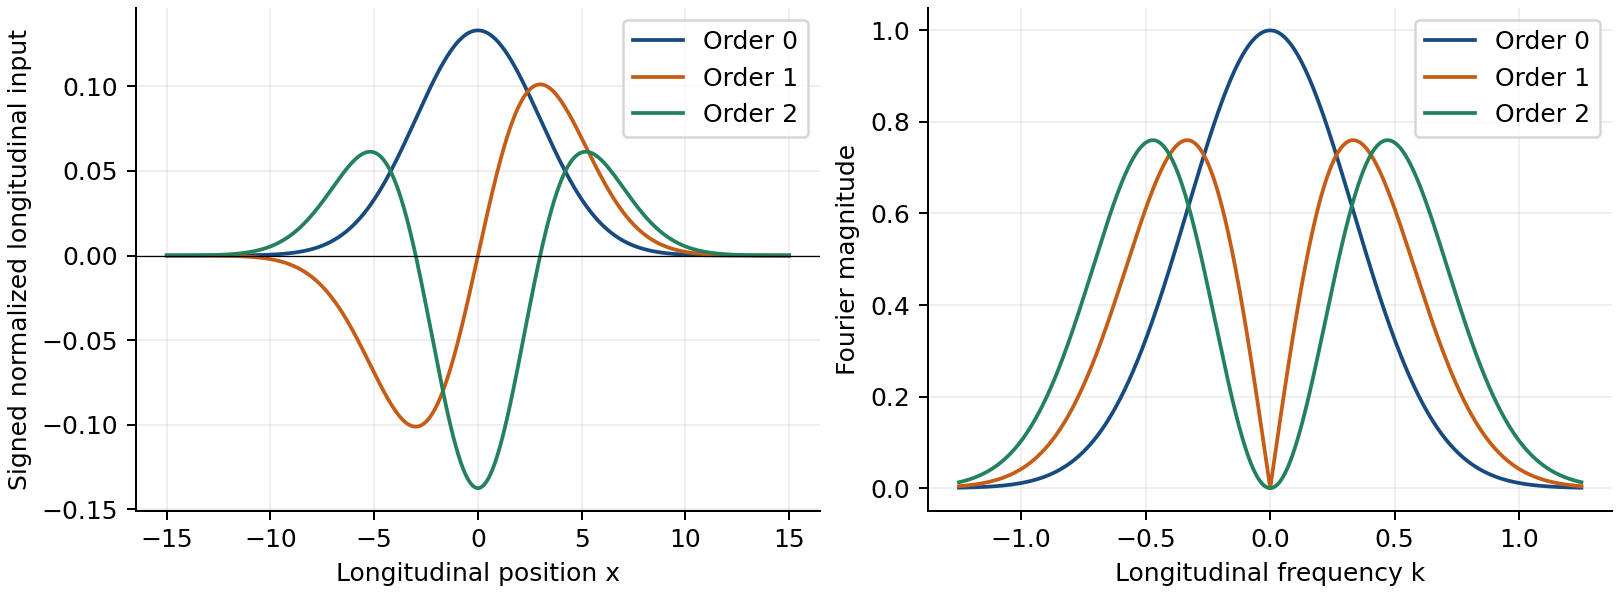
\includegraphics[width=\linewidth]{inputs.png}
\caption{Longitudinal input factors at width $3$ and their Fourier magnitudes. Signed cancellation is visible on the left; its low-frequency suppression is visible on the right. Every full three-coordinate input has $L^1$ norm one.}
\end{figure}

Cancellation alone does not remove the scaling obstruction. If $f$ has these vanishing moments, so does $f_\lambda(X)=\lambda^3f(\lambda X)$. Moreover,
\[
 M_{f_\lambda}(t)=\lambda^{7/2}M_f(\lambda^3t).
\]
An unrestricted bound $M_f(t)\leq Ct^{-\gamma}\|f\|_1$ on this rescaling-invariant class would force $\gamma\leq7/6$. To seek a faster estimate, one must introduce an additional scale-sensitive norm or restriction. For example, $\int |X|^j|f(X)|\,dX$ changes by $\lambda^{-j}$ under this scaling. Such a norm may support a different inequality; its sufficiency still requires analysis.

\newpage
\section{A spectral gap: avoid the degenerate plane}
For the homogeneous symbol,
\[
 \det D^2\omega=216k(k^2+\ell^2+n^2).
\]
Its Hessian is nonsingular away from $k=0$. This motivates a smooth spectrum with fixed separation from that plane. Define
\[
 b_q(k)=\begin{cases}
 \exp\!\left(1-\dfrac{1}{1-((k-q)/h)^2}\right),& |k-q|<h,\\
 0,& |k-q|\geq h,
 \end{cases}\qquad h=\tfrac14.
\]
The two inputs have Fourier transform
\[
 \widehat f_q(k,\ell,n)=\frac{b_q(k)}{B}e^{-9(\ell^2+n^2)/2},
 \qquad q=0\ \hbox{or}\ q=\tfrac34.
\]
Here $B$ is the $L^1$ norm of the inverse longitudinal transform, computed numerically. Modulation preserves that norm, so the two bands use the same $B$. The inverse-transform normalization changes by approximately $5.1\times10^{-6}$ relatively when its integration grid and period are refined.

The centered control occupies $-1/4<k<1/4$. The separated band occupies $1/2<k<1$, and therefore excludes the degenerate plane exactly. This is a smooth compact longitudinal band, not a Gaussian merely centered away from zero. Its transverse spectrum remains Gaussian rather than compactly supported.
\begin{figure}[!htbp]\centering
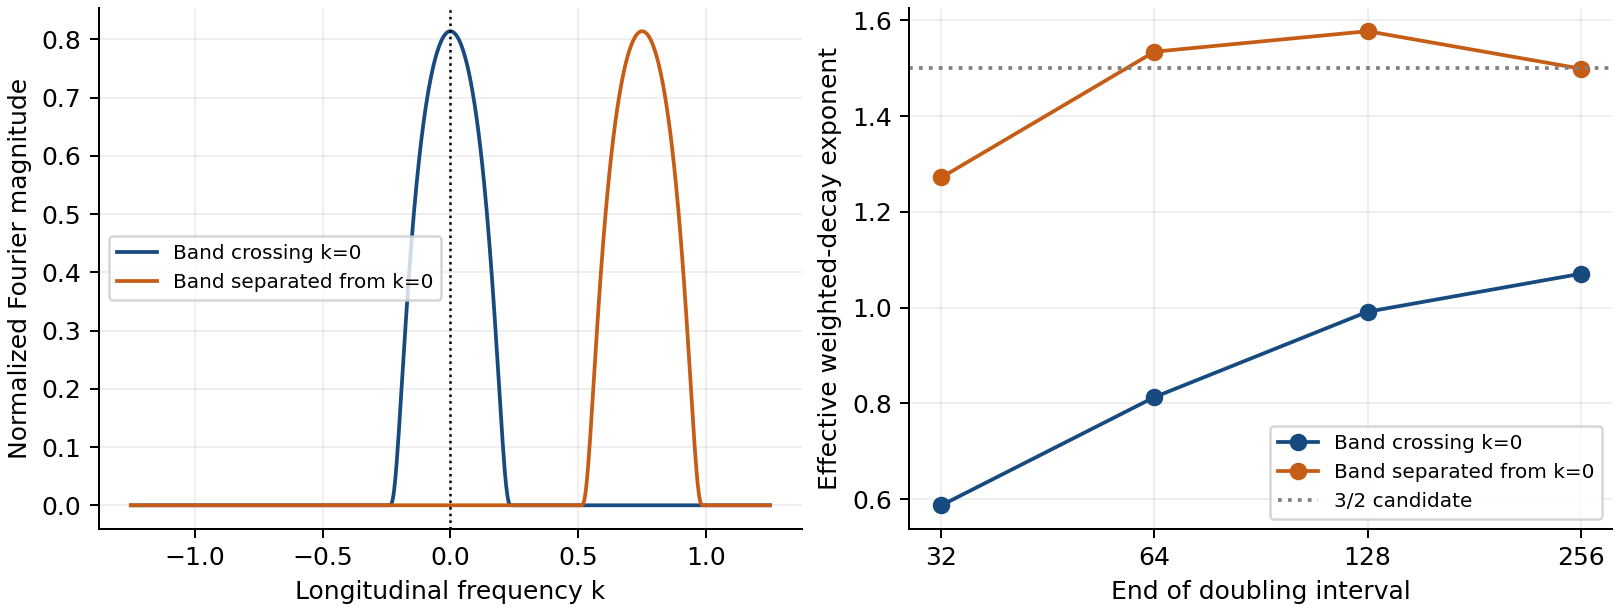
\includegraphics[width=\linewidth]{gap.png}
\caption{Same band shape, different spectral location. The separated band approaches an effective exponent of $3/2$ in the tested intervals. The centered control has slower finite-interval decay. These are numerically normalized artificial inputs.}
\end{figure}

Nondegenerate stationary phase motivates $t^{-3/2}$ as a candidate in three coordinates. A theorem-oriented next class should specify a smooth cutoff supported in a fixed bounded frequency region with $|k|\geq\delta>0$. Constants would depend on the cutoff, the separation $\delta$, and its regularity. This is a proposed analytical route, not a theorem established by these plots. For the inhomogeneous plus symbol, the additional degeneracy set $k(k+\beta)=\ell^2+n^2$ also matters; avoiding $k=-\beta$ alone is insufficient.

\newpage
\section{New numerical results}
\begin{table}[!htbp]\centering
\begin{tabular}{lrrr}\toprule Input & Width $s$ & $p_{[128,256]}$ & $R(256)$\\\midrule
Gaussian & 3 & 1.0438 & 0.009989 \\
Zero mean & 3 & 1.3509 & 0.004534 \\
Two moments & 3 & 1.4935 & 0.002559 \\
Gaussian & 6 & 1.0748 & 0.008880 \\
Zero mean & 6 & 1.2837 & 0.006709 \\
Two moments & 6 & 1.4289 & 0.004894 \\
Band crossing zero & -- & 1.0706 & 0.007473 \\
Separated band & -- & 1.4992 & 0.000761 \\
\bottomrule\end{tabular}
\caption{The eight inputs in the pilot. The last two use a frequency bandwidth rather than the Gaussian width parameter.}
\end{table}
\begin{figure}[!htbp]\centering
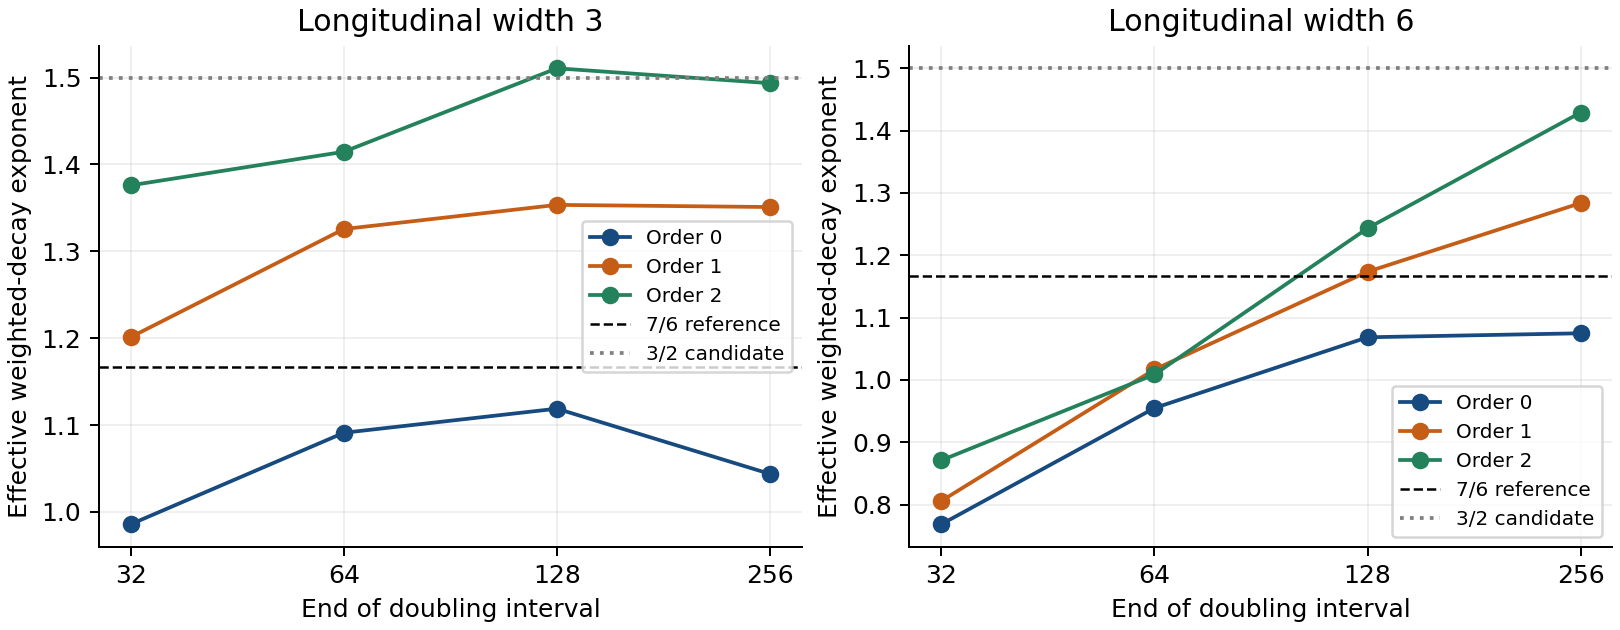
\includegraphics[width=\linewidth]{cancellation.png}
\caption{Cancellation increases the observed decay exponent, but the approach depends on input width. Each marker compares two consecutive times, rather than fitting a single power law over the entire run.}
\end{figure}

The clearest numerical contrast is between the two smooth bands: their widths and normalization agree, while their spectral locations differ. The separated band gives $p_{[128,256]}\approx1.4992$; the centered control gives $1.0706$. This supports prioritizing spectral exclusion for further study.

The cancellation series also supports further work. At width $3$, the final exponent rises from $1.0438$ to $1.3509$ and $1.4935$ as cancellation order increases. At width $6$, the corresponding values are $1.0748$, $1.2837$, and $1.4289$. Width dependence is a direct reason to avoid treating one endpoint slope as the final asymptotic answer.

We have not shown that all zero-mean inputs decay at one common faster rate, that every separated band has exponent exactly $3/2$, or that the original $7/6$ estimate is false. The results concern the homogeneous linear operator and artificial data. No nonlinear or measured-data evolution is part of this batch.

\newpage
\section{Numerical method and reliability}
Analytic transverse Gaussian integration reduces the weighted field to
\[
 W(t,x,r)=\frac{1}{4\pi^2}\int_{\mathbb R}
 \frac{F(k)|k|^{1/2}}{9+6itk}
 \exp\!\left(itk^3+ikx-\frac{r^2}{2(9+6itk)}\right)\,dk,
\]
where $F$ is the appropriate longitudinal spectrum above. Thus the computation retains a three-coordinate field while exploiting radial symmetry. It does not discretize a narrow transverse periodic box.

Each input is evaluated at $16,32,64,128,256$. The search configurations are
\begin{center}\begin{tabular}{lrrrr}\toprule
Search & Longitudinal period & $\Delta x$ & Maximum $r$ & $\Delta r$\\\midrule
Base & 8192 & 0.5 & 512 & 4\\
Longer & 16384 & 0.5 & 512 & 4\\
Finer and wider & 16384 & 0.25 & 1024 & 2\\\bottomrule
\end{tabular}\end{center}
The four largest radial-row candidates seed local optimization in $(x,r)$. At the selected point, a doubled longitudinal period is checked against the original Fourier sum, and an independent adaptive integral evaluates the complex field. Gaussian frequency integration is truncated at twelve standard deviations. Smooth-band integration uses its exact compact support.

The pilot screen requires relative differences below one percent in sampled peaks across the period and grid/radius changes, in the pointwise period comparison, and in the independent complex-field comparison. Boundary magnitude must be below one percent of the candidate peak, and the selected optimizer must report success. This is a numerical screening criterion, not an error bound.

Thirty-eight of forty first-pass records satisfy the screen. At $256$, the separated band has appreciable amplitude at the initial radial boundary; extending to $r=4096$ reduces the checked boundary fraction to roundoff without changing the peak. The centered band initially changes its sampled peak by $1.106\%$ under refinement. A further $\Delta r=1$ search through $2048$ reproduces the finer sampled maximum and the optimized peak. Both follow-ups pass; the original flags remain saved.

Independent Fourier checks of the Hermite inputs agree with their analytic transforms to approximately $3.4\times10^{-16}$ in absolute error. The Gaussian control reproduces the existing solver at a common test point to roundoff. These checks verify normalization and operator consistency; they do not exclude a narrow peak missed between all search points.

The next numerical audit should extend all eight inputs through $512$ and $1024$, retain the enlarged radial searches, and tighten the screen to $0.1\%$. Spectral-gap width and separation should then vary independently, with several smooth cutoff shapes and small controlled leakage into the excluded band. A fixed-input plateau is more informative than a single favorable exponent.

\newpage
\section{Making the model practical for fluids}
The canonical three-coordinate linear model answers a mathematical dispersion question. A practical water experiment requires the water-wave equation's own coordinates, amplitudes, and assumptions. Our existing one-profile-coordinate spatial Dysthe implementation is a useful first validation target: a probe measures a time record at one position, and the model predicts records at downstream positions. It cannot represent arbitrary directional spreading across a basin. The spatial formulation and its wave-envelope interpretation are described by Fedele and Dutykh~\cite{FD}; laboratory comparisons using measured upstream records have an established precedent~\cite{Shemer}.

\subsection{Restore units before comparing with a laboratory}
For a declared deep-water carrier, set
\[
 \omega_0=2\pi/T_0,\quad k_0=\omega_0^2/g,\quad
 c_g=\omega_0/(2k_0),\quad \epsilon=k_0a_{\rm ref}.
\]
In the convention already used in our spatial report,
\[
 \xi=\epsilon^2 k_0x_{\rm phys},\qquad
 \tau=\epsilon(2k_0x_{\rm phys}-\omega_0t_{\rm phys}),
\]
\[
 \eta_{\rm phys}\simeq\frac{\epsilon}{k_0}
 \operatorname{Re}\{u(\xi,\tau)e^{i(k_0x_{\rm phys}-\omega_0t_{\rm phys})}\}.
\]
The last formula is a leading-harmonic reconstruction. Bound harmonics and mean-flow corrections must be treated consistently when comparing detailed crest heights. At a fixed gauge, $\tau$ decreases as laboratory time increases; preprocessing must respect this sign and the carrier convention.

As an illustrative design, take $T_0=0.8$ seconds, $a_{\rm ref}=0.008$ metres, $g=9.81$ metres per second squared, and depth $0.6$ metres. The deep-water formulas give $k_0\approx6.29$ inverse metres, wavelength approximately $1.00$ metre, $\epsilon\approx0.0503$, and $k_0h\approx3.77$. One unit of $\xi$ is approximately $62.9$ metres, while one unit of $\tau$ at a fixed gauge is approximately $2.53$ seconds in magnitude. These are illustrative choices, not fitted experimental parameters. They show why a numerical endpoint cannot simply be read as seconds or metres. Depth effects must be checked against $\omega_0^2=gk_0\tanh(k_0h)$ for the selected experiment.

\subsection{A concrete validation sequence}
\begin{enumerate}
\item Choose a narrow-band, nonbreaking, nearly unidirectional record with known depth, gauge positions, time units, elevation units, and sampling rate.
\item Remove instrumental offsets, identify the carrier, and extract a complex envelope with a documented filter and analytic-signal convention. Retain the original elevation record. Check sensitivity to filtering and window edges.
\item Normalize from the physical carrier and amplitude scale. Use only the upstream gauge to define the input; do not fit the downstream records that will serve as validation.
\item Predict downstream gauge histories using the existing spatial Dysthe solver. Compare with a linear control and an NLS control under the same input and measurement convention.
\item Report errors in envelope magnitude, carrier phase or arrival time, peak elevation, and spectrum, alongside grid/box/time-step refinement and measurement uncertainty. A good-looking surface alone is insufficient.
\end{enumerate}

\newpage
\section{A candidate dataset and the next research decisions}
A public candidate is Lande's 2026 DataverseNO collection~\cite{Lande}. It contains wave-gauge and paddle records spanning linear to breaking groups, with flat-bed and shoal configurations. The stated still-water depth is $0.6$ metres, and the dataset is released under CC BY 4.0. The associated publication is listed as under review. We have inspected the public catalog, not imported or validated a gauge record.

The appropriate first subset would be a nonbreaking flat-bed case, subject to checking bandwidth and depth compatibility. Shoaling or breaking cases must not be presented as valid applications of the existing constant-depth weakly nonlinear deep-water solver. The catalog alone is insufficient to select a final run; record-level metadata and data quality must be inspected first.

Practical calibration and restricted-input analysis should inform one another without being conflated. Exact cancellation and hard spectral exclusions are controlled mathematical experiments. Measured envelopes contain noise and leakage. A useful robustness experiment is therefore
\[
 f_\eta=\frac{f_{\rm gap}+\eta g_{\rm low}}{\|f_{\rm gap}+\eta g_{\rm low}\|_1},
 \qquad \eta=0,10^{-4},10^{-3},10^{-2},
\]
where $g_{\rm low}$ is a fixed low-frequency contaminant. Its phase and amplitude must be specified. This tests how long the apparently faster regime survives when the restriction is imperfect. It is proposed work, not a completed measurement in this report.

For nonlinear solitary-wave experiments, the total peak need not decay. The appropriate future decay observable is the radiation after a carefully defined phase-and-position fit to a solitary component. Pulse-core persistence, radiative decay, and conservation diagnostics should be reported separately. Subtracting an arbitrary fitted curve can manufacture apparent decay, so the fitting rule and its sensitivity must be explicit.

The immediate priorities are: extend and tighten the present restricted-input audit; test spectral leakage and fixed-gap parameter families; and import one suitable laboratory record into the dimensional spatial solver. These tasks address different questions and should produce separate claims. A successful linear spectral-gap experiment is not, by itself, validation of a physical nonlinear water model.

\section{Reproduction and saved evidence}
Run the following from the project root:
\begin{verbatim}
python verify_restricted_decay.py
python restricted_decay.py
python refine_restricted_decay.py
python report/build_restricted_report.py
\end{verbatim}
The verification command checks the inputs and baseline operator independently. The simulation command reuses existing per-case records. Refinement retains first-pass flags and appends follow-ups. The final command regenerates figures and the result table. Raw search parameters, complex-field comparisons, optimizer status, and follow-ups are stored under \texttt{results/restricted\_decay/}. The report source and figures compile independently of simulation arrays. Earlier reports and simulations are preserved.

\begin{thebibliography}{9}
\bibitem{FD} F. Fedele and D. Dutykh, Hamiltonian form and solitary waves of the spatial Dysthe equations, JETP Letters 94 (2011), 840--844. arXiv:1110.4083.
\bibitem{Shemer} L. Shemer, A. Sergeeva, and A. Slunyaev, Applicability of envelope model equations for simulation of narrow-spectrum unidirectional random wave field evolution: Experimental validation, Physics of Fluids 22 (2010), 016601. doi:10.1063/1.3290240.
\bibitem{Lande} O. Lande, Background Data for: A laboratory experiment and procedure for deterministic validation of numerical wave models, DataverseNO, version 1 (2026). doi:10.18710/FZN3AL. Catalog accessed 16 September 2026.
\end{thebibliography}
\end{document}
